% =============================================================
%  MIMIC-IV Septic Shock EWS: Exploratory Analysis Report
%  Compiled with XeLaTeX / pdfLaTeX (requires booktabs, graphicx,
%  amsmath, hyperref, geometry, caption, subcaption, natbib)
%
%  Revision 2026-03-28 (rerun all steps; T1.1–T1.4 incorporated):
%    · Table 1: analysable vs excluded baseline comparison
%    · Table 2: primary conditional logistic regression
%    · Table S1–S4: standard/GEE, dedup, bootstrap, late-vitals sensitivity
%    · Abstract, Discussion, Limitations updated per reviewer comments
% =============================================================
\documentclass[referee,lineno,pdflatex]{sn-article-template/sn-jnl}

% ── packages ──────────────────────────────────────────────────
\usepackage{amsmath, amssymb}
\usepackage{booktabs}
\usepackage{microtype}
\usepackage[numbers,sort&compress]{natbib}
\usepackage{array}
\usepackage{makecell}
\usepackage{tikz}
% sn-jnl.cls defines \orcidlogo via EPS; clear it so orcidlink (texlive 2025)
% can redefine it with its own TikZ implementation (no external image needed).
\makeatletter
\@ifundefined{orcidlogo}{}{\let\orcidlogo\relax}
\makeatother
\usepackage{orcidlink}
\usetikzlibrary{arrows.meta, positioning, calc}
\raggedbottom

% ── title block ───────────────────────────────────────────────
\title[Heart Rate Lag-1 Autocorrelation and Pre-shock Dynamics]{Heart Rate Lag-1 Autocorrelation Is Associated with Pre-shock Dynamics in Late-Onset Septic Shock: A Single-Cohort Exploratory Analysis of MIMIC-IV}

\author[1]{\fnm{Chengyi} \sur{Fang}\,\orcidlink{0009-0006-1237-7763}}\email{f1justin@tongji.edu.cn}
\author*[2]{\fnm{Haiping} \sur{Yu}\,\orcidlink{0000-0002-3394-2841}}\email{pingping670@sina.com}
\author*[3]{\fnm{Qiancheng} \sur{Luo}\,\orcidlink{0000-0003-4054-5593}}\email{luoqiancheng19@163.com}

\affil[1]{\orgname{Tongji University School of Medicine}, \orgaddress{\city{Shanghai}, \country{China}}}
\affil[2]{Department of Nursing, Pudong Gongli Hospital, Shanghai University of Medicine \& Health Sciences, \city{Shanghai}, \country{China}}
\affil[3]{Department of Critical Care Medicine,  Pudong Gongli Hospital, Shanghai University of Medicine \& Health Sciences, \city{Shanghai}, \country{China}}

% ==============================================================
\begin{document}
\maketitle
\label{strobe:item1a}% STROBE item 1(a): study design in title (title page)

% ==============================================================
\begin{abstract}

\textbf{Background.}
Septic shock carries in-hospital mortality exceeding 40\%, yet current severity scores
capture the absolute magnitude of physiological derangement rather than the dynamic
regulatory capacity that declines before haemodynamic collapse.
In hourly electronic health record (EHR) data, rising heart-rate lag-1 autocorrelation
(AC1) may reflect \emph{physiological rigidity} (progressive loss of cardiovascular
regulatory flexibility) rather than high-frequency critical slowing down per se.

\noindent
\textbf{Methods.}
From MIMIC-IV v3.1, we identified 41,296 Sepsis-3 ICU stays; 10,310 met an operational
septic shock definition (vasopressor plus lactate $>$2\,mmol/L plus $\geq$1\,L crystalloid).
Risk-set matching (1:2, admission SOFA $\pm$2) yielded 2,172 analysable matched pairs
(725 shock, 1,447 control).
Rolling 12-h variance (MAP) and HR AC1 were computed over a 48-h pre-event observation period after
a 24-h detrending burn-in.
Primary comparisons used early- and late-centred window summaries with clustered GEE and
global Holm correction; the primary adjusted analysis used conditional logistic regression
stratified by matched pair and adjusted for ventilation, ICU type, monitoring modality,
sedative, and beta-blocker exposure.

\noindent
\textbf{Results.}
HR AC1 was significantly elevated in shock in the late-centred window
(0.382 vs.\ 0.323; Holm $p<0.001$) but not in the early window (Holm $p=0.316$).
The LMM time-by-group interaction was positive ($\beta=0.00143$, $p=0.024$).
In the primary conditional logistic model, late-centred HR AC1 remained correlated with shock
(OR\,=\,1.60, 95\,\%\,CI\,1.15--2.22, $p=0.005$); sedative exposure showed the strongest
independent association (OR\,=\,4.70, 3.73--5.93, $p<0.001$).
After additional adjustment for concurrent mean MAP and HR, the HR AC1 term was not
significant (OR\,=\,1.23, 0.85--1.78, $p=0.271$).
GEE and deduplicated-subset sensitivity analyses reproduced the primary estimate
(OR\,=\,1.61 and 1.65, respectively).
The association was absent in the no-sedation subgroup (OR\,=\,1.07, $p=0.815$) and
attenuated under double detrending (OR\,=\,1.29, $p=0.159$).
MAP variance showed no robust late-centred group difference.

\noindent
\textbf{Conclusions.}
HR AC1 is elevated in the near-event phase of late-onset septic shock and remains
significant after care-setting adjustment, but does not survive concurrent vital-sign
adjustment.
These findings support HR AC1 as a marker of late physiological rigidity co-evolving with
haemodynamic deterioration, rather than as an independent occult early-warning signal.



\label{strobe:abstract}% STROBE item 1(b): abstract summary
\end{abstract}
\keywords{late-onset septic shock, MIMIC-IV, critical slowing down, autocorrelation, early warning signal, physiological rigidity, conditional logistic regression}

% ==============================================================
\section{Background}
\label{sec:intro}

Septic shock is among the most time-critical syndromes in critical care,
with in-hospital mortality exceeding 40\% despite modern management \cite{singer2016}.
Current severity scores---SOFA, APACHE, SAPS---as well as routine vital-sign monitoring,
primarily reflect the absolute magnitude of physiological derangement rather than the
dynamic regulatory capacity of the cardiovascular system.
Yet before vasopressor initiation or overt haemodynamic collapse, patients often undergo
a period of progressive loss of cardiovascular regulatory flexibility that these indices
alone may fail to capture.

Among the variables continuously monitored in the ICU, heart rate (HR) is the most
immediately available, non-invasive readout of cardiovascular autonomic function:
it is recorded continuously at the bedside without additional equipment, is not acutely
confounded by vasopressor titration as mean arterial pressure is, and is available at
every charting interval in the electronic health record.
During the progression of sepsis, systemic inflammatory response and endothelial injury
severely impair autonomic nervous system (ANS)-mediated cardiovascular homeostasis
\cite{decastilho2018,adam2023}.
This regulatory failure manifests as increasing \emph{physiological rigidity}: HR
progressively loses its adaptive responsiveness to physiological demands---failing, for
instance, to accelerate appropriately with fever or to recover promptly after
resuscitation---and the system's ability to return to baseline following perturbations
slows.

This pattern of slowing recovery and declining resilience as haemodynamic reserve is
exhausted is consistent with what complex dynamical systems theory describes as
\emph{Critical Slowing Down (CSD)} \cite{scheffer2009,dakos2012}.
CSD provides a mathematical framework for quantifying such physiological rigidity at the
bedside: its core statistical signature is rising lag-1 autocorrelation (AC1), reflecting
a system increasingly locked to its prior state and unable to respond flexibly
\cite{scheffer2009}.
AC1 is directly computable from the HR time series available in any monitored ICU patient.
Applying this framework to clinical medicine, Olde Rikkert et al.~\cite{olderikkert2016}
proposed that slowing of recovery and rising autocorrelation constitute generic risk
markers for acute severity transitions across a range of chronic diseases, providing a
conceptual basis for translating CSD indicators into critical care practice.
Khalil et al.~\cite{khalil2025} identified HR~AC1 as the primary significant CSD
indicator before ICU extubation failure, suggesting the principle may extend to other
forms of haemodynamic deterioration; Chen et al.~\cite{chen2012} found that rising
intra-system correlation broadly characterises the pre-transition state in complex
diseases.
However, both lines of evidence relied on second-resolution waveform data or non-septic
populations.

In most ICUs, hourly nurse-charted EHR vital signs are the practical data standard---far
below the sampling rates used in prior CSD-ICU work.
Whether EHR-resolution HR~AC1 can serve as a warning signal before haemodynamic
deterioration specifically in septic shock has not been examined in a large,
methodologically controlled cohort.
We therefore conducted an exploratory matched-cohort analysis using MIMIC-IV
\cite{johnson2023} to assess whether hourly EHR-derived HR~AC1 is elevated before
late-onset septic shock and to clarify its relationship with concurrent illness severity.

% ==============================================================
\section{Methods}
\label{sec:methods}

\subsection{Data source}
MIMIC-IV version 3.1 was accessed under the PhysioNet Data Use Agreement.
Derived concepts (SOFA, suspicion of infection, vasopressor equivalents)
were generated using the official MIT \texttt{mimic-code} DuckDB SQL pipeline
\cite{johnson2023}.

\subsection{Cohort construction}
\label{sec:cohort}

\paragraph{Sepsis-3 definition.}
ICU stays satisfying Sepsis-3 criteria \cite{singer2016}---
suspected infection (culture plus antibiotic within 24--72\,h)
and SOFA score $\geq 2$---were extracted from the
\texttt{mimiciv\_derived.sepsis3} table, yielding 41,296 eligible stays.

\paragraph{Septic shock definition.}
An operational definition was applied:
among all vasopressor initiations (norepinephrine, epinephrine, dopamine,
phenylephrine, vasopressin; \texttt{inputevents} item IDs 221906, 221289, 221662,
221749, 222315) within the ICU stay,
we required at least one lactate measurement $>$2\,mmol/L
within a $\pm$24-hour interval around vasopressor start
(lactate \texttt{itemid}s: 50813, 52442, 53154),
vasopressor duration of at least 1\,hour,
and at least 1\,L isotonic crystalloid in the preceding 24\,hours
(\texttt{NaCl 0.9\%}, \texttt{Lactated Ringer's solution (LR)}, or \texttt{dextrose 5\% in LR (D5LR)}).
The earliest qualifying vasopressor time was designated $T_0$.
This identified 10,310 shock stays.
As a design-sensitivity check, the corresponding shock counts were 9,239 using
$\pm$6\,h and 9,909 using $\pm$12\,h intervals, indicating modest cohort-size
sensitivity to this operational choice.
Adequate fluid resuscitation was approximated from recorded crystalloid volume as a
pragmatic proxy for a prospectively adjudicated resuscitation endpoint.

\paragraph{Risk-set matching.}
For each shock patient, the elapsed time to $T_0$ from ICU admission ($H$) was computed.
Before matching, we pre-screened each candidate analysis window for downstream
analysability: candidates required at least 72\,h ICU observation before $T_0$
(to support a 24\,h burn-in period plus a 48\,h analysis window) and at least
24 actual hourly MAP observations and 24 actual hourly HR observations in the
final 48\,h before $T_0$.
The eligible control pool was constructed as a \emph{dynamic} risk set.
Specifically, Sepsis-3 stays were eligible if their ICU duration was $\geq H$ hours
and their own shock onset (if any) occurred \emph{after} time $H$.
This design allows patients who later developed shock to serve as
\emph{future-shock controls} prior to their own $T_0$.
Up to two controls were drawn per case (seed 42) matched on admission SOFA $\pm$2
(1:2 ratio selected to increase statistical efficiency relative to 1:1 matching
while preserving match quality \cite{austin2010}),
with pseudo-$T_0 =$ \texttt{icu\_intime} $+ H$.
After this pre-screen, 725 shock stays were matchable and yielded 1,450 matched control
observations (2,175 total matched pairs; unique controls used up to 3 times).
All downstream analyses use the matched (stay, $T_0$) pair as the analysis unit.

\subsection{Time-series extraction and preprocessing}
\label{sec:preprocessing}

Hourly MAP (ABPm: item 220052; NBPm: item 220181, merged by preference)
and HR (item 220045) were extracted for the 72-hour period preceding each $T_0$.
Monitoring modality (ABPm- vs.\ NBPm-dominant: $>$70\% of readings from one source)
was labelled for sensitivity analysis using only measurements within the final
48\,h analysis window.
Preprocessing:
\begin{enumerate}
  \item Physiological range filtering: MAP between 30 and 200\,mmHg; HR between 20 and 300\,bpm (values outside these ranges were treated as implausible artefacts and excluded).
  \item Resampling to 1-hour bins (median aggregation).
  \item Causal detrending using a trailing 24-hour mean.
    The first 24\,h of the 72\,h extraction were used only as burn-in so that every
    analysed hour in the final 48\,h had a fully populated trailing baseline.
  \item $\mu \pm 3\sigma$ outlier replacement (within-patient).
  \item Exclusion: stays with $<$24 actual (non-interpolated) data points in the
    final 48\,h analysis window.
\end{enumerate}
Of 2,175 matched (stay, $T_0$) pairs, 2,172 (99.9\%) passed preprocessing;
the pre-screening step therefore moved almost all data-quality exclusion upstream.

\subsection{EWS computation}
\label{sec:ews}

Two sliding-window indicators were computed over the 48-hour post-burn-in residual series:
\begin{description}
  \item[Variance-MAP] Rolling standard deviation of MAP residuals
    (CSD predicts rising variance in a \emph{regulated} variable \cite{rector2021}).
  \item[AC1-HR] Rolling lag-1 Pearson autocorrelation of HR residuals.
\end{description}
Window: 12\,hours; step: 1\,hour; $\approx$37 window values per patient.
Each rolling window was indexed by its midpoint time rather than its end time;
with a 48-hour analysable series, realised window centers therefore ranged from
approximately $-42$ to $-5$\,h relative to $T_0$.
For each indicator, windows with fewer than 8 actual (non-interpolated) observations
of \emph{that indicator} were flagged as low-confidence and excluded from that
indicator's comparisons independently.
MAP data sparsity does not filter HR windows and vice versa.
For AC1-HR, autocorrelation was additionally computed only from valid adjacent point
pairs (i.e.\ consecutive 1-hour bins both containing real observations);
windows with fewer than 8 such pairs were set to missing and excluded from all
downstream comparisons.

\subsection{Primary statistical analysis}
\label{sec:stats}

For each (stay, $T_0$) pair, three summaries were extracted for each indicator:
an early-centred rolling-window mean (window centers $-48$ to $-24$\,h),
a late-centred rolling-window mean (window centers $-12$ to $<0$\,h),
and a within-pair late-minus-early change.
Between-group comparisons:
\begin{itemize}
  \item Early-centred rolling-window mean: Gaussian GEE with \texttt{stay\_id} clustering.
  \item Late-centred rolling-window mean: Gaussian GEE with \texttt{stay\_id} clustering.
  \item Late-minus-early change: Gaussian GEE with \texttt{stay\_id} clustering.
\end{itemize}
To reduce multiplicity from subgroup exploration, Holm--Bonferroni correction was
applied globally across the full-cohort and monitoring-modality subgroup comparisons.
Temporal divergence was additionally assessed with a linear mixed-effects model (LMM):
\texttt{indicator $\sim$ time * group + (1 + time | pair)}, where \texttt{pair}
denotes the matched analysis unit.

\subsection{Baseline table}
\label{sec:stats-table1}

Baseline characteristics were compared between shock and control rows within the
analysable matched cohort ($725$ shock, $1{,}447$ control).
Variables included: age, sex, race, admission SOFA, ICU length of stay, ICU type
(first care unit), respiratory support before $T_0$, vasopressor use before
$T_0$, hospital mortality, and monitoring modality.
Continuous variables: Wilcoxon rank-sum test; summary as median [IQR].
Categorical variables: chi-square (Fisher's exact when expected cell count $<$5).
Standardised mean difference (SMD) was computed for each variable
(Cohen's $d$ for continuous; Austin--Stuart formula for binary \cite{austin2015}).

\subsection{Primary matched multivariable analysis}
\label{sec:stats-model}

To test whether HR~AC1 is associated with shock after adjusting for
care-setting covariates while respecting the matched design, conditional logistic
regression stratified by \texttt{matched\_pair\_id} was fitted on analysable pairs with
complete modelling data:
\begin{description}
  \item[Primary model] \texttt{shock $\sim$ ac1\_hr\_late\_mean + vent\_before\_window}\\
    \texttt{+ sedation\_before\_window + betablocker\_before\_window}\\
    \texttt{+ icu\_type + monitoring},
    stratified by matched pair.\\
    Main predictor: mean HR~AC1 across late-centred rolling windows
    (window centers $-12$ to $<0$\,h).
\end{description}
The matched time-from-admission structure and admission SOFA (used as the matching
caliper) are controlled structurally by the matched-pair likelihood and require no
separate coefficient.
Age and sex were neither part of the matching criteria nor included as explicit
covariates, and therefore represent potential sources of residual confounding.
Results are reported as odds ratios (OR) with 95\% confidence intervals.
Unconditional standard logistic regression and stay-level clustered GEE are reported
as sensitivity analyses in Section~\ref{sec:stats-robust}.

\subsection{Cluster-robust and bootstrap sensitivity analyses}
\label{sec:stats-robust}

\paragraph{GEE (T1.3).}
Generalised estimating equations \cite{liang1986} with a logistic link,
exchangeable within-cluster correlation structure, and \texttt{stay\_id} as the
clustering unit were used to refit the adjusted model as a sensitivity analysis.
For comparison, the corresponding unconditional standard logistic model is also
reported. These models do not fully condition on matched-pair strata, but assess
whether the primary association is sensitive to alternative variance structures.

\paragraph{Deduplicated subset (T1.3).}
Each \texttt{stay\_id} was restricted to one randomly selected $T_0$
(seed 42; 2,118\,$\to$\,1,915 analysable rows), reducing repeated observations within stay.
All primary statistical tests were re-run on this subset.

\paragraph{Late-window raw vital-sign sensitivity (T1.2 extension).}
To test whether HR~AC1 simply reflected overt deterioration in conventional vital signs,
the primary conditional logistic model was additionally adjusted for the raw
final-12\,h mean MAP and HR before $T_0$.

\paragraph{Stay-level cluster bootstrap (T1.4).}
To provide distribution-free uncertainty quantification for group-level effect sizes,
a non-parametric stay-level cluster bootstrap was applied:
each unique \texttt{stay\_id} was treated as an indivisible unit; 1,000 stratified
resamples (by group, with replacement) were drawn; all $T_0$ rows belonging to each
sampled stay were carried into the bootstrap sample; for each resample, three
group-difference statistics were computed (late-centred AC1 mean, early-centred AC1 mean,
and early-to-late AC1 change).
Bootstrap 95\% confidence intervals were obtained by the percentile method.

\subsection{Perturbation-recovery analysis (exploratory)}
\label{sec:perturbation}

Routine ``Turn'' events (item 224082)
were used as timestamped physiological perturbations.
MAP recovery area (AUC-recovery) was computed as the integral of
$|\text{MAP}(t) - \text{baseline}|$ over 0--30\,min post-Turn (trapezoid rule);
baseline = preceding 15-min median MAP.
Events were excluded if vasopressor was changed within $\pm$30\,min,
if $<$3 total MAP readings were available across the event window,
or if fewer than two post-Turn recovery points were observed.
Within-group (early $-24$ to $-12$\,h vs.\ late $-6$ to $0$\,h) and
between-group comparisons used Wilcoxon rank-sum on patient-pair-median AUC.
This analysis is designated exploratory.

All analyses were performed in Python 3.14 (\texttt{pandas}, \texttt{numpy},
\texttt{scipy}, \texttt{statsmodels}, \texttt{seaborn}).

% ==============================================================
\section{Results}
\label{sec:results}

\subsection{Cohort characteristics and representativeness}
\label{sec:res-cohort}

Figure~\ref{fig:consort} and Table~\ref{tab:cohort} summarise the cohort construction cascade.
Of 41,296 Sepsis-3 ICU stays, 10,310 (25.0\%) met the stricter operational shock definition.
After upstream data-quality pre-screening and risk-set matching, 725 shock and 1,450 control
(stay, $T_0$) pairs were generated; 725 shock and 1,447 control pairs remained analysable after
time-series cleaning (2,172 total).

\begin{figure}[htbp]
  \centering
  \begin{tikzpicture}[
    node distance = 10mm,
    box/.style  = {draw = black!65, rounded corners = 3pt,
                   fill = blue!6,   text width = 62mm,
                   align = center,  font = \small,
                   inner sep = 5pt, minimum height = 11mm},
    excl/.style = {draw = black!55, rounded corners = 3pt,
                   fill = orange!10, text width = 52mm,
                   align = center,   font = \small,
                   inner sep = 4pt},
    arr/.style  = {-{Stealth[scale=0.9]}, semithick},
    harr/.style = {-{Stealth[scale=0.8]}, black!45},
  ]
    %% ── Main column ──────────────────────────────────────────────
    \node[box] (N1)
      {\textbf{MIMIC-IV v3.1 ICU stays}\\[3pt]$n = 94{,}458$};
    \node[box, below=of N1] (N2)
      {\textbf{Sepsis-3 eligible}\\[3pt]$n = 41{,}296$};
    \node[box, below=of N2] (N3)
      {\textbf{Septic shock -- operational definition}\\[3pt]$n = 10{,}310$};
    \node[box, below=of N3] (N4)
      {\textbf{Pre-screened risk-set pool}\\[2pt]
       {\footnotesize(Sepsis-3 stays; $\geq$72\,h obs.; $\geq$24 hourly MAP/HR readings)}\\[2pt]
       $n_{\text{pool}} = 20{,}690$};
    \node[box, below=of N4] (N5)
      {\textbf{After 1:2 risk-set matching (SOFA\,$\pm$2)}\\[3pt]
       Shock: $n = 725$\quad Control: $n = 1{,}450$};
    \node[box, below=of N5] (N6)
      {\textbf{Analysable matched cohort}\\[3pt]
       Shock: $n = 725$ \textbullet{} Control: $n = 1{,}447$ \textbullet{} Total: $2{,}172$};

    %% ── Vertical arrows ──────────────────────────────────────────
    \draw[arr] (N1) -- (N2);
    \draw[arr] (N2) -- (N3);
    \draw[arr] (N3) -- (N4);
    \draw[arr] (N4) -- (N5);
    \draw[arr] (N5) -- (N6);

    %% ── Midpoints between consecutive nodes ──────────────────────
    \path (N1.south) -- coordinate[midway] (M12) (N2.north);
    \path (N2.south) -- coordinate[midway] (M23) (N3.north);
    \path (N3.south) -- coordinate[midway] (M34) (N4.north);
    \path (N4.south) -- coordinate[midway] (M45) (N5.north);
    \path (N5.south) -- coordinate[midway] (M56) (N6.north);

    %% ── Common left edge for all exclusion boxes ─────────────────
    \coordinate (XL) at ($(N1.east) + (8mm, 0)$);

    %% ── Exclusion boxes ──────────────────────────────────────────
    \node[excl, anchor=west] (E1) at (XL |- M12)
      {Excluded: not meeting\\Sepsis-3 criteria\\$n = 53{,}162$};
    \node[excl, anchor=west] (E2) at (XL |- M23)
      {Excluded: no qualifying vasopressor,\\
       lactate $>$2\,mmol/L, or $\geq$1\,L\\
       crystalloid ($n = 30{,}986$)};
    \node[excl, anchor=west] (E3) at (XL |- M34)
      {Excluded: ${<}$72\,h ICU stay\\
       or insufficient MAP/HR\\observations};
    \node[excl, anchor=west] (E4) at (XL |- M45)
      {Excluded: no eligible 1:2\\match on SOFA\,$\pm$2};
    \node[excl, anchor=west] (E5) at (XL |- M56)
      {Excluded: time-series\\cleaning ($n = 3$ control pairs)};

    %% ── Horizontal branch arrows ─────────────────────────────────
    \draw[harr] (N1.east |- M12) -- (E1.west);
    \draw[harr] (N2.east |- M23) -- (E2.west);
    \draw[harr] (N3.east |- M34) -- (E3.west);
    \draw[harr] (N4.east |- M45) -- (E4.west);
    \draw[harr] (N5.east |- M56) -- (E5.west);
  \end{tikzpicture}
  \caption{%
    \textbf{Participant flow diagram.}
    CONSORT-style flow of ICU stays from the MIMIC-IV v3.1 source database through
    Sepsis-3 eligibility screening, operational septic shock definition, data-quality
    pre-screening, 1:2 risk-set matching, and final time-series cleaning to the
    analysable matched cohort.
  }
  \label{fig:consort}
\end{figure}

\begin{table}[ht]
\centering
\caption{Cohort construction cascade.}
\label{tab:cohort}
\begin{tabular}{lrr}
\toprule
Step & $n$ & \% of prior \\
\midrule
MIMIC-IV v3.1 ICU stays & 94,458 & --- \\
Sepsis-3 eligible & 41,296 & 43.7 \\
Septic shock (operational, stricter) & 10,310 & 25.0 \\
Pre-screened risk-set pool & 20,690 & --- \\
\midrule
\multicolumn{3}{l}{\textit{After upstream pre-screening and final cleaning:}} \\
Shock (stay, $T_0$) pairs & 725 & 7.0 \\
Control (stay, $T_0$) pairs & 1,447 & --- \\
Total analysable & 2,172 & --- \\
\bottomrule
\end{tabular}
\end{table}

\paragraph{Baseline profile (Table~\ref{tab:table1}).}
Table~\ref{tab:table1} describes the analysable matched cohort (shock vs.\ control).
Because downstream preprocessing excluded only three matched pairs, the table characterises
the cohort as a whole rather than providing an analysable-versus-excluded audit.
As expected under risk-set matching, age and admission SOFA were broadly similar between
groups, whereas hospital mortality and pre-$T_0$ vasopressor exposure were substantially
higher in the shock group.

\begin{table}[ht]
\centering
\caption{%
  Baseline characteristics of the analyzable matched cohort.
  Values are median [IQR] or $n$ (\%).%
}
\label{tab:table1}
\begin{tabular}{lrrrrr}
\toprule
Variable &
  \makecell{Shock\\$N=725$} &
  \makecell{Control\\$N=1{,}447$} &
  $p$ & SMD \\
\midrule
\multicolumn{5}{l}{\textit{Demographics}} \\
Age, years            & 65 [54--74] & 63 [54--75] & 0.483 & 0.035 \\
Male sex              & 411 (56.7\%) & 862 (59.6\%) & 0.198 & $-$0.058 \\
\midrule
\multicolumn{5}{l}{\textit{Severity and ICU course}} \\
Admission SOFA        & 6 [4--9] & 6 [4--8] & 0.398 & 0.045 \\
ICU LOS, days         & 13.8 [8.8--22.2] & 12.3 [7.7--19.6] & $<$0.001 & 0.144 \\
Hospital mortality    & 412 (56.8\%) & 308 (21.3\%) & $<$0.001 & 0.782 \\
\midrule
\multicolumn{5}{l}{\textit{Treatment at $T_0$}} \\
Respiratory support before $T_0$ & 630 (86.9\%) & 1,220 (84.3\%) & 0.110 & 0.074 \\
Vasopressor before $T_0$ & 676 (93.2\%) & 599 (41.4\%) & $<$0.001 & 1.326 \\
\midrule
\multicolumn{5}{l}{\textit{ICU type (first care unit)}} \\
MICU                  & 351 (48.4\%) & 627 (43.3\%) & $<$0.001 & 0.102 \\
SICU                  & 177 (24.4\%) & 456 (31.5\%) & --- & $-$0.159 \\
CCU/CSRU              & 162 (22.3\%) & 217 (15.0\%) & --- & 0.189 \\
Neuro/NICU            & 14 (1.9\%)  & 117 (8.1\%)  & --- & $-$0.285 \\
Other                 & 21 (2.9\%)  & 30 (2.1\%)  & --- & 0.053 \\
\midrule
\multicolumn{5}{l}{\textit{Monitoring modality}} \\
ABP-dominant          & 280 (38.6\%) & 543 (37.5\%)  & 0.808 & 0.023 \\
NBP-dominant          & 359 (49.5\%) & 738 (51.0\%) & --- & $-$0.030 \\
Mixed                 & 86 (11.9\%) & 166 (11.5\%)  & --- & 0.012 \\
\bottomrule
\end{tabular}
\begin{tablenotes}
  \item[*] $|$SMD$| \geq 0.1$: meaningful imbalance between groups.
  \item Full Table 1 with race breakdown and complete SMD values is provided in
        \texttt{output/table1\_baseline.csv}.
\end{tablenotes}
\end{table}

\subsection{Primary EWS: HR lag-1 autocorrelation}
\label{sec:res-main}

Results are summarised in Table~\ref{tab:main} and illustrated in
Figures~\ref{fig:timeseries} and~\ref{fig:delta}.

\begin{sidewaystable}[p]
\caption{%
  Between-group comparison of EWS indicators.
  Early/late refer to rolling 12\,h windows indexed by midpoint time.
  Early centers: $-48$ to $-24$\,h. Late centers: $-12$ to $<0$\,h.
  $\Delta$ = late minus early.
  Raw $p$-values are stay-level clustered GEE; Holm correction was applied globally
  across full-cohort and subgroup comparisons.
}
\label{tab:main}
\begin{tabular}{lrrrrrrrrrr}
\toprule
 & \multicolumn{3}{c}{Early-centred mean} & \multicolumn{3}{c}{Late-centred mean} & \multicolumn{3}{c}{$\Delta$ (late $-$ early)} \\
\cmidrule(r){2-4} \cmidrule(r){5-7} \cmidrule(r){8-10}
Indicator & Shock & Control & GEE / Holm $p$ & Shock & Control & GEE / Holm $p$ & Shock & Control & GEE / Holm $p$ \\
\midrule
\textbf{Variance-MAP} & 64.20 & 72.30 & 0.0062 / 0.0685 & 77.00 & 74.99 & 0.5129 / 1.0000 & 12.78 & 2.43 & 0.0016 / 0.0249 \\
\textbf{AC1-HR}       & 0.345 & 0.323 & 0.0395 / 0.3157 & 0.382 & 0.323 & $<$0.001 / $<$0.001 & 0.036 & $-$0.002 & 0.0208 / 0.1872 \\
\bottomrule
\end{tabular}
\footnotetext{Full cohort: shock $n=725$; control $n=1{,}447$.}
\end{sidewaystable}

HR~AC1 was the clearest dynamic signal.
The early-window HR~AC1 difference was modest (0.345 vs.\ 0.323; raw $p=0.0395$)
and did not survive global Holm correction.
By contrast, the late-centred difference was pronounced
(0.382 vs.\ 0.323; Holm $p<0.001$).
The within-pair late-minus-early change was also larger in shock
(0.0356 vs.\ $-0.0018$), although this contrast did not remain significant after
global multiplicity correction.
The complementary LMM gave a positive time-by-group interaction for HR~AC1 in the
full cohort ($p=0.0241$), supporting a gradual steepening of the near-event trajectory sampled by the late-centred windows.

MAP variance showed a different pattern: no corrected late-centred difference was present
in the full cohort, but the late-minus-early increase was larger in shock
(12.78 vs.\ 2.43; Holm $p=0.0249$).
Because this signal was not accompanied by a corrected late-centred separation or by an
LMM interaction, MAP variance was retained as a secondary finding only.
The time-series plot (Figure~\ref{fig:timeseries}, upper panel) shows largely
overlapping MAP variance trajectories, with the shock group rising sharply only at
$T_0$ itself (a likely consequence of haemodynamic collapse rather than an early warning).

\begin{figure}[ht]
  \centering
  
\includegraphics[width=\linewidth]{output/fig1_timeseries.png}
  \caption{%
    \textbf{EWS time-series (48 hours pre-event).}
    Thin lines and shaded bands show group-mean ($\pm$95\,\% CI) of MAP variance (upper)
    and HR~AC1 (lower) for shock (red) and control (blue) groups; thick lines show
    LOESS-smoothed trends (bandwidth $= 0.3$) to aid visualisation of temporal divergence.
    Vertical dashed line: $T_0$. Green dotted line: early-window-center boundary ($-24$\,h).
    Orange dotted line: late-centred-window boundary ($-12$\,h).
    The upper panel shows a right-skewed MAP variance distribution in both groups,
    reflecting that elevated haemodynamic instability is concentrated in a minority of
    time windows rather than being uniformly distributed; the sharp rise at $T_0$ likely
    reflects haemodynamic collapse rather than an early warning.
    HR~AC1 diverges mainly in the near-event late-centred interval, whereas MAP variance
    shows broader overlap.
  }
  \label{fig:timeseries}
\end{figure}

\begin{figure}[ht]
  \centering
  
\includegraphics[width=0.7\linewidth]{output/fig2_delta_boxplot.png}
  \caption{%
    \textbf{Distribution of early-to-late change.}
    Shock group (red) vs.\ control (blue) for both indicators.
    HR~AC1 shows a rightward shift in shock, indicating greater late-centred elevation.
  }
  \label{fig:delta}
\end{figure}

\subsection{Primary matched analysis after covariate adjustment}
\label{sec:res-model}

Table~\ref{tab:model} presents the primary matched conditional logistic regression
results ($n = 2{,}059$ observations across 695 informative matched strata with
complete data).
The late-centred rolling-window HR~AC1 summary remained associated with shock after conditioning on the
matched-pair structure and adjusting for within-stratum care-setting covariates:
OR\,=\,1.60 (95\,\%\,CI\,1.15--2.22, $p = 0.005$).
Because the conditional likelihood absorbs stratum-specific intercepts, matched
features such as admission SOFA and time-from-admission are controlled by design
rather than re-estimated as separate coefficients.
Sedative exposure in the prior 12\,h showed the strongest within-stratum association
with shock (OR\,=\,4.70, 3.73--5.93; $p<0.001$), whereas beta-blocker exposure was
not clearly associated (OR\,=\,0.68, 0.45--1.02; $p=0.065$).
The primary AC1 estimate was directionally stable in unconditional logistic and GEE
sensitivity analyses (Table~S1), suggesting that the result is not driven solely by
ignored within-stay clustering.
However, after additional adjustment for raw final-12\,h MAP and HR, the HR~AC1 term
was attenuated and no longer significant
(OR\,=\,1.23, 0.85--1.78; $p = 0.271$; Table~S4).

\begin{table}[ht]
\centering
\caption{%
  Primary multivariable conditional logistic regression for late-onset septic shock
  ($n = 2{,}059$ observations; 695 informative matched strata).
  OR: odds ratio; 95\,\% CI: Wald confidence interval.
  Reference categories: MICU (ICU type), NBP-dominant (monitoring modality).
  Matching variables and stratum-specific intercepts are conditioned out by design.
  Unconditional standard logistic and GEE sensitivity analyses are reported in Table~S1;
  late-vitals-adjusted sensitivity is reported in Table~S4.
  $\dagger$: primary predictor of interest.%
}
\label{tab:model}
\begin{tabular}{lrr}
\toprule
Variable & OR (95\,\% CI) & $p$ \\
\midrule
\textbf{HR AC1, late-centred window mean}$^\dagger$ & \textbf{1.60 (1.15--2.22)} & \textbf{0.005} \\
Invasive MV at $-12$\,h  & 0.70 (0.55--0.89) & 0.004 \\
Sedation exposure in prior 12\,h & 4.70 (3.73--5.93) & $<$0.001 \\
Beta-blocker exposure in prior 12\,h & 0.68 (0.45--1.02) & 0.065 \\
ICU type: SICU vs MICU & 0.68 (0.53--0.88) & 0.004 \\
ICU type: CCU/CSRU vs MICU & 1.55 (1.16--2.06) & 0.003 \\
ICU type: Neuro/NICU vs MICU & 0.29 (0.15--0.55) & $<$0.001 \\
ICU type: Other vs MICU & 0.82 (0.43--1.58) & 0.561 \\
Monitoring: ABP vs NBP & 0.93 (0.73--1.19) & 0.549 \\
Monitoring: Mixed vs NBP & 1.07 (0.76--1.51) & 0.695 \\
\bottomrule
\end{tabular}
\end{table}

\subsection{Sensitivity analysis: monitoring modality}
\label{sec:res-sensitivity}

Figure~\ref{fig:subgroup} shows the main time-series for
ABPm-dominant ($n_s = 280$, $n_c = 543$) and NBPm-dominant
($n_s = 359$, $n_c = 738$) subgroups.
Late-window HR~AC1 remained higher in shock in both subgroups after global Holm correction
(ABPm Holm $p=0.0357$; NBPm Holm $p=0.0275$), although the subgroup LMM interaction
was not significant for ABPm and was only borderline for NBPm ($p=0.0579$).

\begin{figure}[ht]
  \centering
  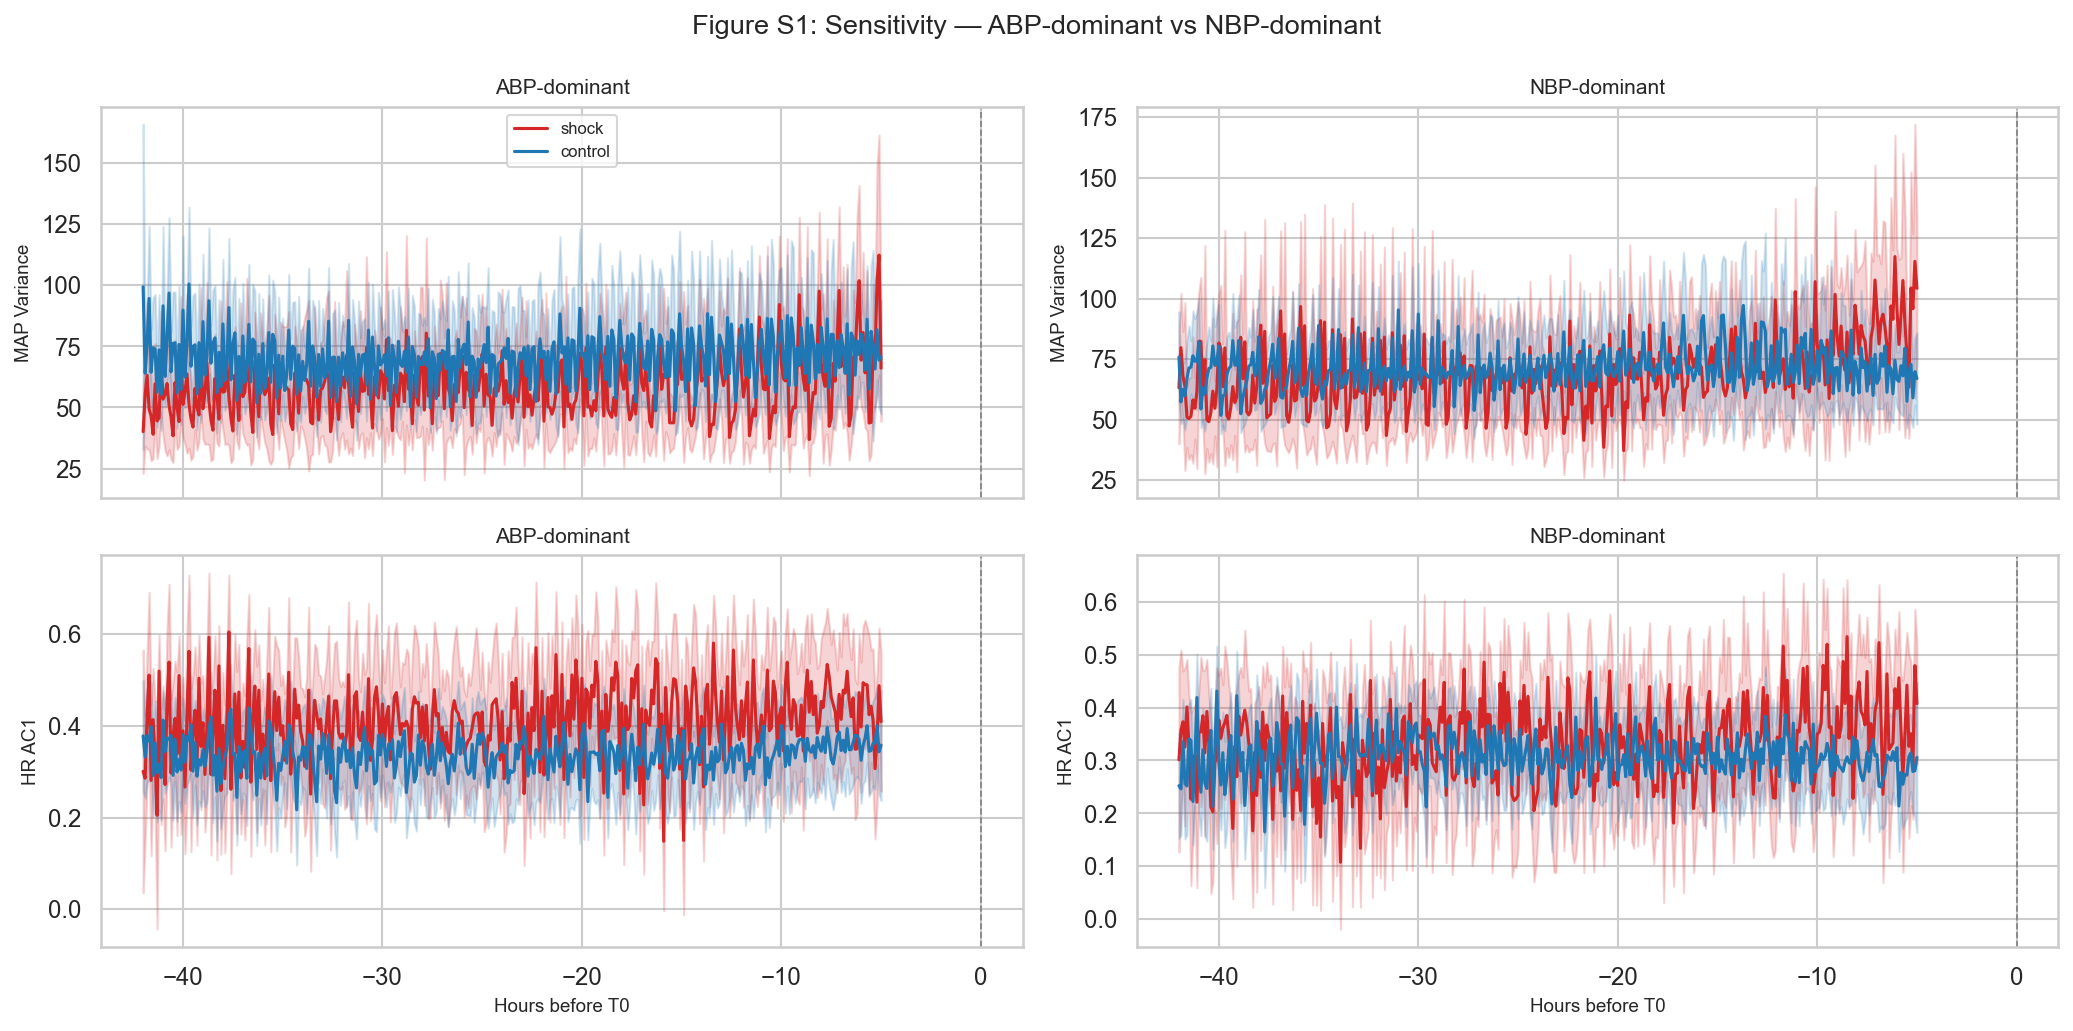
\includegraphics[width=\linewidth]{output/figS1_subgroup.png}
  \caption{%
    \textbf{Sensitivity analysis: ABPm-dominant (left) vs.\ NBPm-dominant (right) subgroups.}
    MAP variance (top) and HR~AC1 (bottom).
    The HR~AC1 elevation in shock persists across both monitoring modalities.
  }
  \label{fig:subgroup}
\end{figure}

\subsection{Cluster-robust and bootstrap sensitivity}
\label{sec:res-robust}

\paragraph{GEE (Table S1).}
Fitting GEE with \texttt{stay\_id} as the clustering unit and exchangeable correlation
structure, the adjusted OR for the late-centred HR~AC1 summary was 1.61 (1.17--2.22, $p=0.003$).
The corresponding unconditional standard logistic estimate was 1.63 (1.18--2.25, $p=0.003$).
Both were very close to the primary conditional logistic estimate
(OR\,=\,1.60, 1.15--2.22), indicating that the association is not driven solely by
ignored within-stay clustering or by the matched-strata parameterisation.

\paragraph{Deduplicated subset (Table S2).}
Restricting to one randomly selected $T_0$ per \texttt{stay\_id}
(2,118\,$\to$\,1,915 analysable rows)
reproduced the primary direction of findings:
the late-centred HR~AC1 summary remained higher in shock (Wilcoxon $p<0.001$),
early-to-late HR~AC1 change also remained larger in shock ($p=0.012$),
and the adjusted logistic estimate was unchanged
(OR\,=\,1.65, 1.18--2.31, $p=0.003$).

\paragraph{Bootstrap 95\% CIs (Table S3).}
All three key statistics had bootstrap 95\% CIs excluding zero:
$\Delta$late-centred AC1 [0.0331, 0.0862];
$\Delta$early-window AC1 [0.0033, 0.0465];
$\Delta$early-to-late AC1 change [0.0041, 0.0647].
These intervals support a consistent though modest shift of HR~AC1 upward in shock,
including a measurable difference even in the early window.

\paragraph{Final-12\,h raw vital-sign sensitivity (Table S4).}
Because conventional vital signs were already abnormal in the final 12\,h before $T_0$,
we additionally adjusted the primary conditional logistic model for raw final-12\,h
mean MAP and HR.
The HR~AC1 association no longer remained significant
(OR\,=\,1.23, 0.85--1.78, $p=0.271$),
indicating that the late-centred AC1 summary is not robustly separable from concurrent mean-level MAP/HR
abnormality once both are entered into the same matched model.

\paragraph{Early-window and no-sedation sensitivity (Tables S5--S6).}
When the predictor itself was moved to the early window and the model was adjusted for
raw early-window MAP and HR, HR~AC1 was not independently associated with shock
(OR\,=\,1.12, 0.73--1.72, $p=0.612$; Table~S5A).
By contrast, the late-centred HR~AC1 summary remained associated after adjustment for these earlier
raw vital signs alone (OR\,=\,1.48, 1.05--2.08, $p=0.025$; Table~S5B),
indicating that the late-centred signal is not explained solely by abnormalities already
visible in the earlier mean-level MAP/HR profile.
However, in the subgroup without sedative exposure in the prior 12\,h,
the late-centred HR~AC1 summary was not significant
(OR\,=\,1.07, 0.59--1.95, $p=0.815$; Table~S6),
so the present data do not establish a robust sedation-free AC1 effect.

\paragraph{Double-detrending sensitivity.}
To test whether incomplete detrending might inflate HR~AC1 through residual low-frequency
drift, we repeated the full pipeline after adding a 12-hour trailing local linear
detrending step on top of the primary 24-hour trailing-mean detrending.
In that re-analysis, the full-cohort late-centred AC1 separation remained present in the
window-summary comparison (Holm $p=0.0209$), but the matched conditional logistic estimate
was attenuated and no longer significant (OR\,=\,1.29, 0.91--1.83, $p=0.159$).
Further adjustment for raw final-12\,h MAP and HR again removed the signal
(OR\,=\,0.92, 0.62--1.38, $p=0.701$).
These results suggest that the descriptive late-centred AC1 elevation is not erased by
more aggressive detrending, but its adjusted matched-association is not fully robust to
this specification change.

\subsection{Exploratory: nursing perturbation recovery}
\label{sec:res-perturbation}

After excluding events with vasopressor changes within $\pm$30\,min, sparse recovery series,
or fewer than two post-Turn recovery points, 660 valid Turn events were identified
(involving 330 patients / 340 matched pairs).
The within-shock-group comparison between late ($-6$ to $0$\,h) and early
($-24$ to $-12$\,h) segments did not reach significance
(median AUC 180.0 vs.\ 127.6\,mmHg$\cdot$min; Wilcoxon rank-sum $p = 0.075$),
nor did the between-group comparison (shock vs.\ control in the late segment:
$p = 0.330$; no-vasopressor subgroup: $p = 0.062$; see Figure~S1 in the Supplementary Material).
This analysis is hypothesis-generating only and provides no evidence to support
a physiological resilience interpretation at hourly EHR resolution.

% ==============================================================
\section{Discussion}
\label{sec:discussion}

\subsection{Principal finding}

This single-cohort exploratory analysis demonstrates that HR~AC1 is associated with
pre-shock dynamics over a 48-hour observation period.
Notably, in our risk-set-matched cohort enriched for late-onset septic shock, this
association persisted after matched conditional analysis adjusting for care-setting covariates.
The finding is consistent with Khalil et al.~\cite{khalil2025}
identification of HR~AC1 as a sensitive dynamic summary in ICU data,
and extends it to a more tightly filtered administrative EHR cohort.
From the perspective of Rector et al.~\cite{rector2021},
HR as an effector variable might theoretically show reduced rather than increased AC1
(reflecting adaptive decompensation rather than CSD in a regulated variable).
In hourly EHR data, the present results are best interpreted as evidence of
late \emph{physiological rigidity}: as haemodynamic reserve is exhausted,
HR appears to lose adaptive flexibility and becomes increasingly locked to a narrower,
slower-changing trajectory.
Importantly, this should be framed as a marker of the overt deterioration phase,
not as proof that HR~AC1 provides a fully independent occult warning signal before
conventional vital signs become abnormal.

\subsection{Association after covariate adjustment}

A key concern is whether elevated HR~AC1 is simply a surrogate for admission severity
(i.e.\ high-SOFA patients have less heart-rate variability).
The matched conditional analysis addresses this partially: after conditioning on the
matched-pair structure and adjusting for ventilation status at the start of the late-centred interval,
ICU type, monitoring modality, sedative exposure, and beta-blocker exposure,
HR~AC1 remained associated with shock (OR\,=\,1.60, $p = 0.005$).
Because admission SOFA and time-from-admission were already built into the matching
design, they were controlled structurally rather than through an explicit regression
coefficient.
Unconditional standard logistic and GEE analyses yielded very similar estimates
(OR\,=\,1.63 and 1.61, respectively; both $p = 0.003$),
and the bootstrap provided complementary evidence that effect sizes were non-zero
across resampled datasets.
These results suggest that the HR~AC1 association is not fully explained by selected
care-setting and pharmacological covariates.
However, the very strong sedative association (OR\,=\,4.70) indicates that drug-related
management intensity is itself tightly coupled to the pre-shock state and likely accounts
for part of the observed HR dynamics.
Accordingly, the adjusted association should be interpreted as showing incomplete
independence from measured care-setting covariates rather than definitive independence
from clinical management or concurrent physiological deterioration.
This caution is reinforced by the no-sedation subgroup analysis, in which the late-centred
HR~AC1 term was no longer significant (Table~S6).
That negative result may partly reflect reduced sample size (526 observations across
212 informative strata), but it weakens any strong claim that the observed association
is robustly present in the absence of sedative exposure.

\subsection{Relation to absolute vital-sign deterioration}

A key interpretive challenge is that the late-centred rolling-window summaries are drawn
from a near-event interval that overlaps substantially with the final 12\,h before
vasopressor initiation, when conventional vital signs are already abnormal.
The full-cohort early-window HR~AC1 difference was small and not significant after
global correction (Holm $p = 0.3157$), whereas the late-centred separation was clear
(Holm $p<0.001$).
This pattern indicates that the signal is concentrated in the clinically overt
late deterioration window rather than in a silent preclinical phase.
Accordingly, the present findings should be interpreted as describing a
\emph{near-event deterioration interval sampled by the late-centred windows}, not a silent preclinical phase.
However, the additional sensitivity model adjusting for these raw final-12\,h means
no longer retained an HR~AC1 association (OR\,=\,1.23, $p = 0.271$; Table~S4),
suggesting that the clinically relevant information in the late-centred AC1 summary may overlap
substantially with contemporaneous mean-level MAP and HR abnormalities.
In that sense, HR~AC1 appears to co-evolve with mean-level haemodynamic deterioration.
Therefore, it may be most useful as an additional descriptor of late physiological rigidity,
rather than a standalone occult signal separable from routine bedside vital signs.
The early-window sensitivity analysis is consistent with this interpretation:
once raw early-window MAP and HR were included, early-window HR~AC1 itself was not
independently associated with shock (Table~S5A).
At the same time, the late-centred HR~AC1 summary remained significant when adjusted only for early
raw MAP and HR (Table~S5B), suggesting that the main signal emerges later than these
earlier mean-level covariates rather than functioning as a clear occult warning signal
within the early window itself.
However, the double-detrending re-analysis weakens confidence that the adjusted late-centred
association is fully independent of low-frequency residual trend, because the matched
conditional estimate no longer remained significant under that stricter preprocessing
choice.

\subsection{MAP variance as a secondary indicator}

MAP variance showed mixed evidence across the three comparison dimensions.
The only corrected full-cohort signal was a larger late-minus-early increase in shock
(Holm $p = 0.0249$), while the late-centred mean itself was not different.
This inconsistency suggests that any MAP-variance signal is weaker and less clinically
direct than the HR~AC1 pattern, and is likely to be more dependent on sampling density
than a truly robust bedside marker.

\subsection{Perturbation-recovery: negative exploratory result}

Under the patient-pair-level aggregation design, neither the
within-shock-group time comparison ($p = 0.075$) nor the between-group comparison
($p = 0.330$) reached significance.
This negative result is in contrast to earlier event-level analyses that used
pseudo-replication; the corrected analysis is the definitive estimate.
The perturbation-recovery analysis is therefore best viewed as hypothesis-generating only.
Turn-induced perturbations in principle offer a direct window into haemodynamic resilience,
but their prognostic potential in this cohort is likely constrained by the hourly EHR
temporal resolution: with MAP charted at $\sim$1-hour intervals, each 30-minute recovery
window yields at most a handful of data points, fundamentally limiting recovery-curve
characterisation.
Continuous waveform data would be needed to properly evaluate this approach.

\subsection{Limitations}
\label{sec:limits}

\paragraph{Pre-screening and transportability.}
The key design change in this revision was to move data-quality screening upstream into
cohort construction.
This removed most downstream attrition (2,175 matched pairs entering extraction,
2,172 retained), but at the cost of selecting a narrower late-onset, heavily monitored
population from the outset.
Findings therefore apply primarily to continuously monitored ICU patients with long
pre-event observation windows, not to abrupt early-collapse presentations.

\paragraph{Operational shock definition.}
Although stricter than the earlier vasopressor\,$\pm$\,lactate rule, the present
definition remains an operational approximation of Sepsis-3 shock.
Recorded crystalloid volume is an imperfect proxy for adequate fluid resuscitation.
We chose 1,000\,mL in the preceding 24\,h as an operational lower bound to balance
definition strictness against sample retention in MIMIC-IV, not as a claim that this
fully represents guideline-concordant resuscitation for all body sizes.
Some short-lived or non-septic vasopressor episodes may therefore still be retained,
and some included patients may have undergone only partial fluid resuscitation.
The choice of a $\pm$24\,h lactate coexistence interval also affects cohort size
(9,239 shocks at $\pm$6\,h; 9,909 at $\pm$12\,h; 10,310 at $\pm$24\,h).
A cohort-size sensitivity analysis for stricter crystalloid thresholds showed a monotonic
reduction in shock stays from 10,310 at 1.0\,L to 9,839 at 1.5\,L, 9,369 at 2.0\,L,
8,829 at 2.4\,L, and 8,124 at 3.0\,L, illustrating the trade-off between stricter fluid
requirements and retained sample size.

\paragraph{Non-independent observations.}
A control patient may appear in up to three matched pairs.
For this reason, the primary adjusted model used conditional logistic regression
stratified by matched pair.
We additionally examined GEE (OR\,=\,1.61), a deduplicated subset (OR\,=\,1.65),
and stay-level cluster bootstrap CIs, all of which supported the primary finding.

\paragraph{Late-window clinical deterioration.}
Because the anchor $T_0$ is vasopressor initiation rather than the first biological
moment of haemodynamic compromise, the near-event interval sampled by the late-centred
rolling windows likely includes patients who are already clinically deteriorating and may
already meet bedside criteria for shock.
The observed lower MAP and higher HR in shock pairs support this interpretation.
Our results therefore should not be framed as evidence for a hidden warning signal
that precedes routine vital-sign abnormalities, but rather as an association observed
within the late pre-treatment / pre-vasopressor phase.

\paragraph{Drug confounding remains only partially controlled.}
This revision incorporated explicit covariates for common sedatives and beta-blockers,
and sedative exposure emerged as one of the strongest predictors of shock.
Nevertheless, dose timing, cumulative burden, arrhythmias, and paced rhythms remain
incompletely characterised, so pharmacological and rhythm-related confounding cannot
be considered resolved.

\paragraph{Hourly resolution remains a major limitation.}
Even after replacing the MK framework with early/late summaries and LMM,
the underlying data still consist of hourly nurse-charted observations rather than
continuous waveforms.
This coarse sampling fundamentally limits mechanistic interpretation and likely pushes
the signal toward a marker of late instability rather than an early tipping-point detector.
The double-detrending sensitivity analysis reinforces this concern: more aggressive
low-frequency trend removal weakened the matched adjusted HR~AC1 association, indicating
that mechanistic claims about rigidity versus residual trend cannot be considered resolved
with hourly EHR data alone.

\paragraph{Single-cohort, retrospective design.}
These findings are derived from a single administrative EHR database
using retrospectively computed vital-sign time series.
MIMIC-IV \texttt{chartevents} records nurse-charted values at $\sim$1-hour intervals,
not continuous waveforms; parameters were rescaled from higher-frequency studies,
but reduced information content fundamentally limits sliding-window precision.

\subsection{Future directions}

Priority for future work:
(1)~prospective validation in a high-frequency waveform cohort to overcome
the 1-hour EHR resolution limitation;
(2)~explicit characterisation of beta-blocker, sedative, arrhythmia, and pacing
confounders in a pharmacologically annotated cohort;
(3)~temporal external validation (train 2008--2017, test 2018--2022) to assess
transportability before any clinical application is considered;
(4)~a predictive modelling framework (landmark analysis) to translate association
findings into decision-support metrics with calibrated probabilities.

% ==============================================================
\section{Conclusion}
\label{sec:conclusion}

In a selected subset of continuously monitored MIMIC-IV sepsis patients enriched for
late-onset shock, HR~lag-1 autocorrelation is associated with a near-event late-centred
deterioration over a 48-hour observation period and remains significant in a matched conditional analysis
that includes sedative and beta-blocker covariates.
Standard logistic, GEE, deduplicated-subset, and bootstrap sensitivity analyses all
reproduced the late-centred HR~AC1 association.
However, the signal is concentrated in the near-event late-centred phase, the full-cohort
early-window difference is weak after multiplicity correction, and the HR~AC1 term is no
longer significant after adjustment for raw final-12\,h MAP and HR.
Early-window HR~AC1 was also not independently associated after adjustment for early raw
MAP and HR, and the no-sedation subgroup did not confirm a robust late-centred effect.
Under double detrending, the matched adjusted late-centred association was further
attenuated and no longer significant.
MAP variance provided only secondary and internally inconsistent supporting evidence.
Nursing-perturbation recovery dynamics were hypothesis-generating but insufficient
to establish a between-group signal.
These findings support HR~AC1 primarily as a marker of late physiological rigidity that
co-evolves with overt haemodynamic deterioration, not as an independently actionable
silent-phase alarm.
These single-cohort exploratory results motivate further validation with
high-frequency waveform data, pharmacological confounder control,
and temporal external validation before any clinical deployment is considered.

% ==============================================================
\backmatter

\bmhead{Acknowledgements}
The data used in this study are from MIMIC-IV version~3.1 \cite{johnson2024mimiciv},
hosted on PhysioNet \cite{goldberger2000}.
We thank the researchers at the MIT Laboratory for Computational Physiology and
Beth Israel Deaconess Medical Center for making this resource publicly available.

\section*{Declarations}

\subsection*{Ethics approval and consent to participate}
This study is a secondary analysis of MIMIC-IV version~3.1
\cite{johnson2024mimiciv,johnson2023}, a de-identified, publicly available
critical care database.
The original data collection at Beth Israel Deaconess Medical Center was
approved by the Institutional Review Board (IRB) of the Massachusetts Institute
of Technology and Beth Israel Deaconess Medical Center, which granted a waiver
of informed consent owing to the retrospective and de-identified nature of the
data.
Access to MIMIC-IV was obtained by C.F.\ under PhysioNet's Credentialed Health
Data Licence following completion of the required CITI Program human research
protection training.
No additional IRB approval was required for this secondary analysis of
de-identified records.

\subsection*{Consent for publication}
Not applicable. All data are fully de-identified; no individual patient data
are presented.

\subsection*{Availability of data and materials}
MIMIC-IV v3.1 is freely available via PhysioNet
(\url{https://physionet.org/content/mimiciv/}) under the PhysioNet
Credentialed Health Data Licence; derived patient-level data are not
redistributed per the Data Use Agreement.

\subsection*{Competing interests}
The authors declare that they have no competing interests.

\subsection*{Funding}
\label{strobe:funding}% STROBE item 22
No funding was received for this work.

\subsection*{Authors' contributions}
C.F.: Conceptualization, Methodology, Software, Formal analysis, Data
curation, Writing -- original draft, Visualization, Writing -- review \& editing.
H.Y.: Conceptualization, Supervision, Writing -- review \& editing.
Q.L.: Validation, Supervision, Writing -- review \& editing.
All authors read and approved the final manuscript.

\subsection*{Code availability}
All analysis scripts are openly available at
\url{https://github.com/F1Justin/septic-shock-ews-mimic4} under the MIT
License.

% ==============================================================
\bibliographystyle{sn-article-template/bst/sn-vancouver-num}
\bibliography{references}

% ==============================================================
\bmhead{Supplementary information}

\clearpage
\noindent\textbf{Supplementary Material}

\renewcommand{\thefigure}{S\arabic{figure}}
\renewcommand{\thetable}{S\arabic{table}}
\renewcommand{\theHfigure}{S\arabic{figure}}
\renewcommand{\theHtable}{S\arabic{table}}
\setcounter{figure}{0}
\setcounter{table}{0}

\begin{figure}[ht]
  \centering
  
\includegraphics[width=\linewidth]{output/fig3_recovery.png}
  \caption{%
    \textbf{MAP recovery after nursing Turn events (exploratory).}
    Mean ($\pm$95\,\% CI) MAP deviation from baseline for shock (left)
    and control (right).
    Blue: early ($-24$ to $-12$\,h); red: late ($-6$ to $0$\,h).
    Neither the within-shock-group late vs.\ early comparison ($p = 0.075$)
    nor the between-group comparison ($p = 0.330$) was significant at patient-pair level.
    This analysis is designated exploratory; see Section~\ref{sec:res-perturbation}.
  }
  \label{fig:recovery}
\end{figure}

\end{document}
